\documentclass{article}
\usepackage[preprint]{neurips_2026}

\usepackage[utf8]{inputenc}
\usepackage[T1]{fontenc}
\usepackage{hyperref}
\usepackage{url}
\usepackage{booktabs}
\usepackage{amsfonts}
\usepackage{amsmath}
\usepackage{microtype}
\usepackage{xcolor}
\usepackage{graphicx}
\hypersetup{hidelinks}

% This is an ES 678 course paper, not a conference submission.
\makeatletter
\renewcommand{\@noticestring}{ES 678 Course Project}
\makeatother

% All numbers below are macros generated from results/ by scripts/make_paper_assets.py
% generated by scripts/make_paper_assets.py; do not edit
\newcommand{\biasDevGated}{+0.4}
\newcommand{\biasLockedGated}{+0.0}
\newcommand{\binADev}{0.40}
\newcommand{\binALocked}{0.00}
\newcommand{\binBDev}{3.81}
\newcommand{\binBLocked}{2.74}
\newcommand{\binCDev}{1.89}
\newcommand{\binCLocked}{1.60}
\newcommand{\binDDev}{1.48}
\newcommand{\binDLocked}{0.76}
\newcommand{\binEDev}{1.80}
\newcommand{\binELocked}{0.43}
\newcommand{\binNADev}{472}
\newcommand{\binNALocked}{6}
\newcommand{\binNBDev}{7}
\newcommand{\binNBLocked}{1}
\newcommand{\binNCDev}{181}
\newcommand{\binNCLocked}{38}
\newcommand{\binNDDev}{459}
\newcommand{\binNDLocked}{122}
\newcommand{\binNEDev}{100}
\newcommand{\binNELocked}{66}
\newcommand{\blockMedianDev}{1.06}
\newcommand{\blockMedianLocked}{0.79}
\newcommand{\blockWorstDev}{3.78}
\newcommand{\blockWorstLocked}{0.82}
\newcommand{\ciDevHi}{1.69}
\newcommand{\ciDevLo}{0.67}
\newcommand{\ciLockedHi}{0.82}
\newcommand{\ciLockedLo}{0.77}
\newcommand{\covDev}{67}
\newcommand{\covLocked}{82}
\newcommand{\covLockedVOne}{86}
\newcommand{\delayDev}{0.7}
\newcommand{\delayLocked}{1.0}
\newcommand{\detEpDev}{20}
\newcommand{\detEpLocked}{6}
\newcommand{\dropDev}{33}
\newcommand{\dropLocked}{18}
\newcommand{\fOneAtBad}{0.83}
\newcommand{\fOneAtNative}{0.97}
\newcommand{\falseEpDev}{1}
\newcommand{\falseEpLocked}{0}
\newcommand{\farBaseDev}{0.35}
\newcommand{\farBaseLocked}{0.57}
\newcommand{\farDev}{0.04}
\newcommand{\farLocked}{0.00}
\newcommand{\foneBaseDev}{0.73}
\newcommand{\foneBaseLocked}{0.72}
\newcommand{\foneDev}{0.97}
\newcommand{\foneLocked}{0.99}
\newcommand{\gateHi}{1.7}
\newcommand{\gateLo}{0.55}
\newcommand{\gaugeMax}{55}
\newcommand{\gtEpDev}{21}
\newcommand{\gtEpLocked}{6}
\newcommand{\hancBiasCal}{-9}
\newcommand{\hancBiasPool}{-9}
\newcommand{\hancBiasZero}{+15}
\newcommand{\hancCalN}{30}
\newcommand{\hancDry}{1887}
\newcommand{\hancFrames}{1992}
\newcommand{\hancLowFt}{11.2}
\newcommand{\hancMaeCal}{12}
\newcommand{\hancMaeCalA}{8}
\newcommand{\hancMaeCalB}{11}
\newcommand{\hancMaeCalC}{22}
\newcommand{\hancMaePool}{14}
\newcommand{\hancMaePoolA}{4}
\newcommand{\hancMaePoolB}{7}
\newcommand{\hancMaePoolC}{37}
\newcommand{\hancMaeZero}{20}
\newcommand{\hancMaeZeroA}{19}
\newcommand{\hancMaeZeroB}{13}
\newcommand{\hancMaeZeroC}{24}
\newcommand{\hancN}{39}
\newcommand{\hancOffsetCm}{24}
\newcommand{\hancPeakFt}{18.1}
\newcommand{\hancRangeCm}{211}
\newcommand{\hancTrivial}{86}
\newcommand{\lockedBlocks}{2025-04, 2026-04}
\newcommand{\maeAtBad}{3.61}
\newcommand{\maeAtNative}{1.13}
\newcommand{\maeBaseDevAll}{7.94}
\newcommand{\maeBaseDevGated}{6.97}
\newcommand{\maeBaseLockedAll}{11.67}
\newcommand{\maeBaseLockedGated}{11.52}
\newcommand{\maeBorrowed}{9.82}
\newcommand{\maeDay}{3.41}
\newcommand{\maeDevAll}{3.38}
\newcommand{\maeDevGated}{1.13}
\newcommand{\maeFailGate}{7.90}
\newcommand{\maeHighLap}{4.01}
\newcommand{\maeIR}{3.30}
\newcommand{\maeLockedAll}{3.11}
\newcommand{\maeLockedGated}{0.79}
\newcommand{\maeLockedVOneGated}{1.13}
\newcommand{\maePassGate}{1.13}
\newcommand{\maeRawDev}{1.13}
\newcommand{\maeRawLocked}{0.79}
\newcommand{\maeRegistered}{1.91}
\newcommand{\maeSmoothDev}{1.77}
\newcommand{\maeSmoothLocked}{2.51}
\newcommand{\maeZeroDev}{8.80}
\newcommand{\maeZeroLocked}{18.90}
\newcommand{\marginMaeAtCov}{2.28}
\newcommand{\nBlocks}{15}
\newcommand{\nDevBlocks}{13}
\newcommand{\nDevFrames}{1976}
\newcommand{\nFrames}{2259}
\newcommand{\nLockedBlocks}{2}
\newcommand{\nLockedFrames}{283}
\newcommand{\nearThreeDev}{4.8}
\newcommand{\nearThreeLocked}{2.4}
\newcommand{\nearThreeZeroDev}{3.5}
\newcommand{\nearThreeZeroLocked}{3.7}
\newcommand{\pctBorrowed}{18}
\newcommand{\pctDry}{35}
\newcommand{\pctIR}{25}
\newcommand{\pctOverThree}{65}
\newcommand{\pctRegistered}{82}
\newcommand{\pctThreeBelowPlate}{1}
\newcommand{\plateBottomCm}{4.3}
\newcommand{\plateTopCm}{62}
\newcommand{\precDev}{0.97}
\newcommand{\precLocked}{1.00}
\newcommand{\recBaseDev}{0.74}
\newcommand{\recBaseLocked}{0.57}
\newcommand{\recDev}{0.96}
\newcommand{\recLocked}{0.99}
\newcommand{\regionsMax}{10}
\newcommand{\resBaseA}{6.97}
\newcommand{\resBaseB}{5.66}
\newcommand{\resBaseC}{5.11}
\newcommand{\resBaseD}{5.02}
\newcommand{\resBaseE}{4.97}
\newcommand{\resBaseF}{6.81}
\newcommand{\resBaseG}{11.55}
\newcommand{\resMaeA}{1.13}
\newcommand{\resMaeB}{1.17}
\newcommand{\resMaeC}{1.08}
\newcommand{\resMaeD}{1.23}
\newcommand{\resMaeE}{1.36}
\newcommand{\resMaeF}{1.84}
\newcommand{\resMaeG}{3.61}
\newcommand{\resRmseA}{3.08}
\newcommand{\resRmseB}{3.22}
\newcommand{\resRmseC}{2.96}
\newcommand{\resRmseD}{3.22}
\newcommand{\resRmseE}{3.16}
\newcommand{\resRmseF}{3.82}
\newcommand{\resRmseG}{6.28}
\newcommand{\resSA}{0.16}
\newcommand{\resSB}{0.31}
\newcommand{\resSC}{0.62}
\newcommand{\resSD}{1.2}
\newcommand{\resSE}{2.5}
\newcommand{\resSF}{5.0}
\newcommand{\resSG}{10.0}
\newcommand{\rmseDevGated}{3.1}
\newcommand{\rmseLockedGated}{1.2}
\newcommand{\sDouble}{10.0}
\newcommand{\sFirstBad}{10.0}
\newcommand{\sMaxOk}{5.0}
\newcommand{\sNative}{0.16}
\newcommand{\shallowBaseDev}{8.0}
\newcommand{\shallowBaseLocked}{7.2}
\newcommand{\shallowDev}{2.0}
\newcommand{\shallowLocked}{1.6}
\newcommand{\shallowNDev}{188}
\newcommand{\shallowNLocked}{39}
\newcommand{\shallowZeroDev}{6.9}
\newcommand{\shallowZeroLocked}{7.6}
\newcommand{\sigmaFloor}{3.0}
\newcommand{\sigmaV}{0.55}
\newcommand{\yearFirst}{2023}
\newcommand{\yearLast}{2026}


\title{Reading Shallow Flood Depth from Real USGS Gauge-Camera Footage with a Learned Staff-Plate Reader}

\author{%
  Kalp Shah \\
  Roll Number: 24110152 \\
  Department of Electrical Engineering \\
  Indian Institute of Technology Gandhinagar \\
  \texttt{kalp.shah@iitgn.ac.in}
  \And
  Udit Bhatia \\
  Department of Civil Engineering \\
  Indian Institute of Technology Gandhinagar \\
  \texttt{bhatia.u@iitgn.ac.in}
}

\begin{document}
\maketitle

\begin{abstract}
How accurately can a fixed camera estimate flood water depth, and how does accuracy change with image quality and resolution? I use real USGS gauge cameras with official gauge heights as labels: \nFrames{} frames over \nBlocks{} months from a shallow-flow camera. A learned reader registers each frame, rectifies the staff plate, classifies plate rows as submerged and decodes the water level; an image-quality gate abstains on bad frames. Leaving out whole months, it reaches \maeDevGated\,cm mean absolute error on the \covDev\% of frames passing the gate (\maeBaseDevGated\,cm for a colour-threshold baseline) and \maeLockedGated\,cm on two locked months. Error stays below twice native up to about \resSF\,cm per pixel. A very different river camera is read to \hancMaeCal\,cm over a \hancRangeCm\,cm flood without retraining. Limits: water below the plate bottom is unobservable; transfer evidence is one flood.
\end{abstract}

\section{Problem and Motivation}
\textbf{Question.} Given one frame from a fixed camera that sees a reference object of known scale, estimate the water depth $h$ (cm) at the object. Any flood decision (an alarm threshold, severity classes) is a function of $h$, so I evaluate $h$ itself and report error by depth range rather than fixing a threshold. One row is one frame at one camera and time. The prediction uses the current frame, a one-time setup (reference views, plate geometry) and, for pose recovery only, earlier frames; the gauge is never available at prediction time. Camera water-level work mostly targets rivers or deep urban water \citep{vandaele2021,liang2023}. The main camera (USGS 411229084541101, overland flow near Harlan, Indiana) sees shallow flow, so claims are limited to generalisation across its months, plus one transfer test (Sec.~\ref{sec:limits}).

\section{Data and Preparation}
\textbf{Source.} Frames come from the public USGS National Imagery Management System bucket \citep{nims}; labels are the USGS gage height, both public domain. NWIS was not reachable from my environment, so the gauge values come from the committed result tables of two open-source projects \citep{nims} (not re-checked against NWIS); no camera-derived value is a label. The plate spans 0--\plateTopCm\,cm; the gauge sits beside it.

\textbf{Content.} \nFrames{} frames (median spacing 21\,min), \nBlocks{} month blocks; gauge $-0.6$ to \gaugeMax\,cm; \pctDry\% dry, \pctIR\% infrared night; the pose changes between months.

\textbf{Quality checks.} SIFT registration \citep{sift} to a reference view succeeds on \pctRegistered\% of frames (the rest reuse the last good pose); images show fog, mud or droplets, glare and over-exposure; the plate bottom is at \plateBottomCm\,cm, so shallower water is unobservable.

\textbf{Second camera.} USGS 01421500 (East Branch Delaware River, Hancock NY; portrait view, river staff plate, 11--21\,ft) has \hancFrames{} frames from 2026, but stage rarely reaches its plate: \hancDry{} frames are below it. The July flood (stage \hancLowFt--\hancPeakFt\,ft) gives \hancN{} gated frames on the plate over \hancRangeCm\,cm; \hancCalN{} development frames lie just above the plate bottom.

\textbf{Preprocessing and leakage control.} Frames are resized to 1280\,px; the plate quad is rectified to a $360{\times}48$ strip (row $\approx 0.16$\,cm). Everything learned is fitted on training months only: the dry template (per-row median Lab colour of dry daytime frames), the affine calibration, the classifier, the baseline threshold and the gate thresholds (training Laplacian-variance quantiles). Registration reference views come from development months and use geometry, never labels.

\section{Methods}
\textbf{Baselines.} B0: always 0\,cm. B1: a row is wet if its colour change from the dry template exceeds $\tau$ (tuned on training months), then the decoding below.

\textbf{Learned reader.} For frame $i$ and strip row $k$ (height $h_k$), a gradient-boosted classifier (scikit-learn \texttt{HistGradientBoosting}, \citealp{sklearn}) outputs $p_{ik}=P(\text{row submerged})$ from row colour, change from the template, texture, vertical context and frame quality. Labels are $y_{ik}=\mathbb{1}[h_k<g_i]$ ($g_i$ the gauge height): no manual annotation. Water level is the monotone change point $b^\star=\arg\max_b \sum_{k<b}\log(1-p_{ik})+\sum_{k\ge b}\log p_{ik}$, mapped to height and then to centimetres by a least-squares affine fit; levels at or below the plate bottom report 0. The log-likelihood gap to the runner-up boundary is the confidence \emph{margin}.

\textbf{Transfer to camera 2.} The classifier is trained on camera-1 development months only. For camera 2, the dry template and gate thresholds come from its development months, and the plate quad and nominal scale are read off the printed labels. Three variants: \emph{zero-shot} (nominal geometry), \emph{offset-calibrated} (one level offset fitted on the \hancCalN{} development frames above the plate bottom), and \emph{pooled} (retrained with camera-2 development frames added).

\textbf{Quality gate.} A frame is rejected when the Laplacian variance $v$ of the whole image lies outside $[\gateLo,\gateHi]$ times the training median (low: fog, blur, obstruction; high: lens dirt, droplets, glare).

\section{Evaluation Design}
The split unit is the calendar-month block, never the frame: consecutive frames are near duplicates and lighting and pose are shared within a month. Two blocks (\lockedBlocks) were locked in \texttt{make\_usgs\_splits.py} before any model was trained; the other \nDevBlocks{} (\nDevFrames{} frames) support leave-one-block-out cross-validation (CV) and all tuning (classifier hyperparameters were left at fixed defaults). \textbf{Disclosure:} I looked at the locked blocks twice: the first gate was one-sided, dev errors then showed dirty-lens frames also fail, so the gate became two-sided and the run was repeated (both logged; the first gave \maeLockedVOneGated\,cm at \covLockedVOne\% coverage). It is not a pristine single look.

The July flood is locked for camera 2 and is used for no template, offset or training; each variant is evaluated once. \textbf{Metrics.} Mean absolute error (MAE, primary), RMSE and bias (cm), overall and by gauge depth range (dry $\le 0.5$\,cm, 0.5--10\,cm, $>$10\,cm). Uncertainty is the spread over held-out blocks (95\% intervals bootstrap whole blocks; two locked blocks give none, so locked rows show point values).

\begin{table*}[t]
\centering\small
\caption{Held-out depth error (cm). Gated = frames passing the quality gate (coverage \covDev\% CV, \covLocked\% locked); bias = mean(estimate $-$ gauge); last three columns: MAE by gauge depth range; CI = block bootstrap.}
\label{tab:main}
\begin{tabular}{@{}lllrcccccc@{}}
\toprule
Eval. & Frames & Method & $n$ & MAE [95\% CI] & RMSE & bias & dry & 0.5--10 & $>$10 \\
\midrule
CV & gated & learned reader & 1319 & 1.13 [0.7, 1.7] & 3.1 & +0.4 & 0.4 & 2.0 & 1.5 \\
 & gated & threshold baseline & 1319 & 6.97 [6.0, 8.4] & 10.1 & +1.1 & 5.9 & 8.0 & 7.8 \\
 & all & learned reader & 1976 & 3.38 [2.1, 4.5] & 7.3 & +0.5 & 1.9 & 5.0 & 4.1 \\
\midrule
Locked & gated & learned reader & 233 & 0.79 & 1.2 & +0.0 & 0.0 & 1.6 & 0.6 \\
 & gated & threshold baseline & 233 & 11.52 & 14.6 & -8.7 & 9.2 & 7.2 & 12.5 \\
 & all & learned reader & 283 & 3.11 & 8.9 & -2.1 & 1.6 & 2.1 & 3.4 \\
\bottomrule
\end{tabular}

\end{table*}

\begin{figure*}[t]
\centering
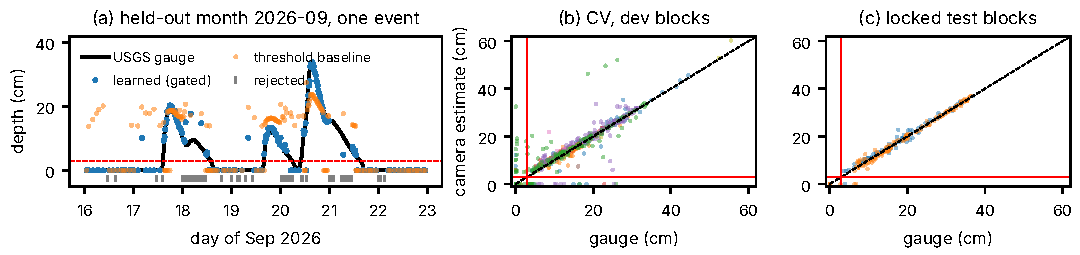
\includegraphics[width=\textwidth]{figs/fig_main.pdf}
\caption{Held-out predictions on real footage. (a) One event in 2026-09 (model never saw this month); grey ticks are rejected frames. (b,c) Camera vs.\ gauge, gated frames, coloured by month.}
\label{fig:main}
\end{figure*}

\section{Results and Error Analysis}
\textbf{Main result.} Table~\ref{tab:main} compares the reader with the baselines (always-0\,cm: \maeZeroDev\,cm CV, \maeZeroLocked\,cm locked). On gated frames in CV the learned reader has \maeDevGated\,cm MAE (95\% CI \ciDevLo--\ciDevHi; RMSE \rmseDevGated, bias \biasDevGated\,cm) versus \maeBaseDevGated\,cm for the threshold baseline. On the two locked months it reaches \maeLockedGated\,cm (baseline \maeBaseLockedGated). Without the gate the errors are \maeDevAll\,cm (CV) and \maeLockedAll\,cm (locked): the gate buys reliability by abstaining on \dropDev\% (CV) and \dropLocked\% (locked) of frames. Per-month MAE has median \blockMedianDev\,cm and worst \blockWorstDev\,cm. (Smoothing hurts: a causal five-reading median raises MAE from \maeRawDev\ to \maeSmoothDev\,cm, since the level moves tens of centimetres per hour; headline numbers are per-frame.)

\textbf{Shallow water.} In the 0.5--10\,cm range (gated CV, $n=\shallowNDev$) MAE is \shallowDev\,cm against \shallowZeroDev\,cm for always-0 and \shallowBaseDev\,cm for the baseline (locked: \shallowLocked, \shallowZeroLocked, \shallowBaseLocked; $n=\shallowNLocked$). That is the largest error relative to depth; below the plate bottom (\plateBottomCm\,cm) depth is unobservable (only \binNBDev{} gated CV frames lie in 0.5--3\,cm).

\textbf{Second camera (Fig.~\ref{fig:main}c).} Zero-shot, the camera-1 classifier reads the Hancock flood with \hancMaeZero\,cm MAE (bias \hancBiasZero\,cm) over \hancN{} frames spanning \hancRangeCm\,cm, against \hancTrivial\,cm for always guessing the plate bottom. One fitted offset (\hancOffsetCm\,cm, \hancCalN{} frames) gives \hancMaeCal\,cm. Pooling camera-2 development frames helps inside the stage range they cover (\hancMaePoolA\ and \hancMaePoolB\,cm at 11--13 and 13--16\,ft vs.\ \hancMaeCalA\ and \hancMaeCalB\,cm) but hurts beyond it (\hancMaePoolC\ vs.\ \hancMaeCalC\,cm at 16--19\,ft): the classifier has seen no water that high on this plate.

\begin{figure*}[t]
\centering
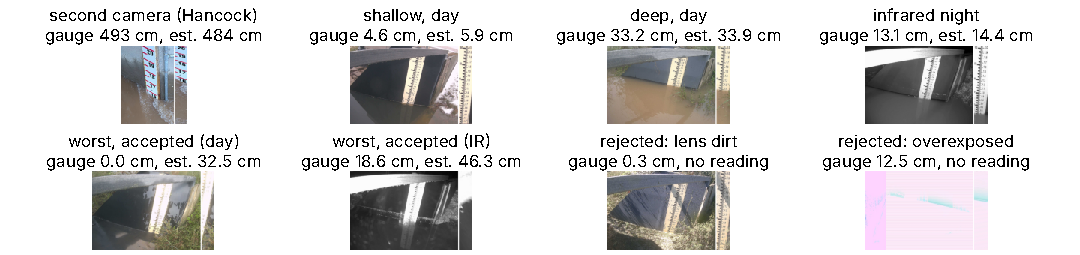
\includegraphics[width=\textwidth]{figs/fig_frames.pdf}
\caption{Real frames (scene crop and rectified plate). Top: median-error examples of each category. Bottom: largest accepted errors and rejected frames. Selection rules are fixed in code (file names in \texttt{paper/figs/fig\_frames\_files.json}).}
\label{fig:frames}
\end{figure*}

\textbf{Failure audit.} Fig.~\ref{fig:frames} (bottom) and the CV subsets show where the error comes from. Infrared is \emph{not} worse than daylight (\maeIR\ vs.\ \maeDay\,cm). Costly cases are a borrowed pose (\maeBorrowed\ vs.\ \maeRegistered\,cm; the camera moved, SIFT failed) and frames outside the gate (\maeFailGate\ vs.\ \maePassGate\,cm). In the worst accepted day frame (gauge 0\,cm) glare washes out the plate and water streaks on the panel look like wet rows; in the worst infrared frame the plate is saturated.


\section{Graduate Depth Analysis}
\textbf{Resolution sweep and error model.} To vary the scale $s$, registration is computed once at native resolution (camera set up once), then each frame is area-downsampled by $f\in\{1,\ldots,64\}$ and the plate re-sampled with $360/f$ rows, giving $s=\sNative f$\,cm/px. (Registering at degraded resolution collapses for $f\ge 8$ and confounds calibration with readout.) The reader is retrained per $f$ with the same CV. Fig.~\ref{fig:depth}a--b: gated MAE is \resMaeA\,cm at the native scale, still \resMaeE\,cm at \resSE\,cm/px and \resMaeF\,cm at \resSF\,cm/px, but \resMaeG\,cm at \resSG\,cm/px, more than twice native; the baseline goes from \resBaseA\ to \resBaseG\,cm. With plate scale $s$ and waterline error $\sigma_v$ (px), $\mathrm{Var}(\hat h)=s^2\sigma_v^2+\sigma_g^2$, where $\sigma_g$ is gauge--plate offset and calibration error. Fitting $\mathrm{RMSE}^2=(\sigma_v s)^2+\sigma_g^2$ to the gated sweep gives $\sigma_v=\sigmaV$\,px and $\sigma_g=\sigmaFloor$\,cm. A sub-pixel $\sigma_v$ is plausible because the change point pools hundreds of rows; the $\sigma_g$ floor dominates at fine scales and reflects gauge offset and residual bad frames. Resolution is therefore not the binding constraint at this camera; the plate bottom and image quality are.

\begin{figure*}[t]
\centering
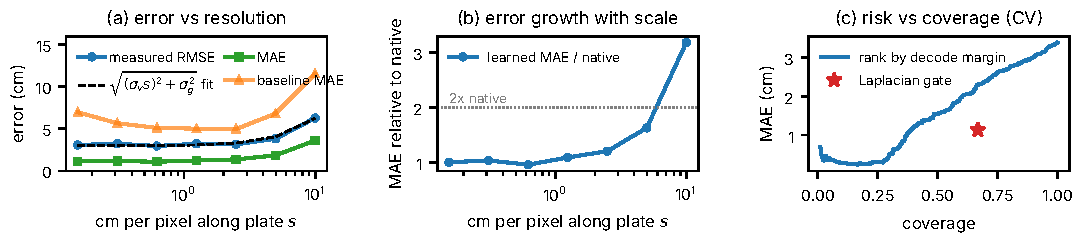
\includegraphics[width=\textwidth]{figs/fig_depth.pdf}
\caption{(a) Depth error vs.\ plate scale $s$ (CV, gated); the dashed line is the fitted error model. (b) Gated MAE relative to its native value. (c) CV MAE vs.\ coverage when ranking frames by decode margin; the gate (star, \maePassGate\,cm) beats margin ranking at equal coverage (\marginMaeAtCov\,cm).}
\label{fig:depth}
\end{figure*}

\section{Limitations and Conclusion}\label{sec:limits}
Camera 1 gives an effective sample size of months, not frames; the transfer evidence is one flood on one other camera (\hancN{} frames). Labels are a gauge beside the plate, not tape measures. The plate begins at \plateBottomCm\,cm, so shallower water is unobservable and reported as 0. The locked set is two months, seen twice, and the gate was designed with dev-month error in view. Stronger claims need more labelled cameras and tape-measured depths.

\textbf{Conclusion.} On real USGS footage a learned plate reader with a quality gate reads depth to about \maeDevGated\,cm (CV) on accepted frames, far better than a colour-threshold baseline, and stays within twice its native error up to about \resSF\,cm/px; it abstains on \dropDev\% of frames and cannot observe depths below \plateBottomCm\,cm.

\section{Reproducibility and AI-Use Disclosure}
Code, splits, gauge tables, the trained model and all results are in \texttt{github.com/kalpshah18/FloodCam} (branch \texttt{main}); \texttt{scripts/make\_paper\_assets.py} regenerates every number, table and figure here from \texttt{results/}. Frames are public domain; no credentials or private data are used. \textbf{AI use:} Claude Code (Anthropic) helped with brainstorming, code, debugging, experiments, the dashboard and drafting. I verified the pipeline with unit tests and by inspecting registration strips, failures and split leakage; I am responsible for all results.

\begin{thebibliography}{9}
\bibitem[Vandaele et~al.(2021)]{vandaele2021} R.~Vandaele et al. River-level monitoring from camera images. \emph{HESS}, 25, 2021.
\bibitem[Liang et~al.(2023)]{liang2023} Y.~Liang et al. V-FloodNet: urban flood video segmentation. \emph{Environ.\ Model.\ Softw.}, 2023.
\bibitem[USGS \& repos(2026)]{nims} U.S. Geological Survey NIMS images and NWIS gage height (public domain); GitHub \texttt{waterline} (Apache-2.0), \texttt{stagesight} (MIT): gauge tables.
\bibitem[Lowe(2004)]{sift} D.~Lowe. SIFT keypoints. \emph{IJCV} 60(2), 2004.
\bibitem[Pedregosa et~al.(2011)]{sklearn} F.~Pedregosa et al. Scikit-learn. \emph{JMLR} 12, 2011.
\end{thebibliography}

\end{document}
